\documentclass[12pt]{article}
\usepackage{booktabs}
\usepackage{geometry}
\usepackage{enumerate}
\usepackage{setspace}
\usepackage{amsthm}
\usepackage{amsmath,amssymb}
\usepackage{amstext}
\usepackage[hidelinks]{hyperref}
\usepackage{graphicx}
\usepackage{setspace}
\usepackage{wrapfig}
\usepackage{fourier}
\usepackage{indentfirst}

\geometry{a4paper,scale=0.82}
\linespread{1.5}

\newtheorem{definition}{Definition}[section]
\newtheorem{theorem}{Theorem}[section]
\newtheorem{lemma}{Lemma}[section]
\newtheorem{proposition}{Proposition}[section]
\newtheorem{remark}{Remark}[section]
\newtheorem{corollary}{Corollary}[section]

\def\d{\mathrm{d}}
\def\Cov{\mathrm{Cov}}
\def\E{\mathrm{E}}
\def\Var{\mathrm{Var}}
\def\unf#1{\textcolor{blue}{#1}}

\newcommand{\HRule}[1]{\rule{\linewidth}{#1}}

\begin{document}

\title{ \normalsize \textsc{VE401 Term Project}
		\\ [3.0cm]
		\HRule{0.5pt} \\ [0.5pt]
        \vspace*{\baselineskip}
		\LARGE \textbf{\textsc{Verification of Sampling Criterion in Testing for Net Quantity of Prepackages with Fixed Content}}
		\HRule{2pt} \\ [0.5cm]
        \vspace*{\baselineskip}
		\normalsize \today \vspace*{5\baselineskip}}

\date{}

\author{
		Project Group 26 \\ 
        \begin{tabular}{ll}
        \normalsize Meng Yuqi & \normalsize 521370910030  \\
        \normalsize Liu Yuzhuo & \normalsize 520021910454  \\ 
		\normalsize Tanchavalit Ekkanat & \normalsize 123  \\
        \normalsize Zhang Maizhe & \normalsize 123  \\
        \end{tabular}}
        

\maketitle
\thispagestyle{empty}
\newpage
\thispagestyle{empty}

\tableofcontents
\newpage
\pagenumbering{arabic}

\section{Abstract}

\newpage

\section{Introduction}

As prepackaged food production becomes prevalent nowadays, inspection on whether the product contains the same amount of content as labeled becomes an important approach to protect the interests of the consumers. However, there are unavoidable errors in the production, which makes it impossible to ensure that every package produced contains content at least as much as what is specified in the label. It would in turn be unfair to the manufacturers as on average they would have to fill more content when packaging the products. Therefore, a statistically reasonable criterion is called for to resolve this dilemma, so that a general agreement is reached upon on how much error is allowable for a certain batch of production; and a standard is derived from the criterion to specify how the random sampling and inspection should be carried out to determine whether the production satisfies the requirement or not.

In our project, we refer to two specific criterion that is published by Chinese government \cite{JJF2005} and International Organization of Legal Metrology \cite{OIML2016}, respectively, to explain how the "statistically reasonable" is established, and verify whether the sampling plan proposed in the two criteria aligns with the requirements that are specified in their materials. We would first look into the \cite{JJF2005} first and cross-validate using \cite{OIML2016}. A comparison between the two criteria will be made; and an empirical sample carried out by ourselves will be demonstrated for supplement. 

\section{Glossary}

In order to avoid confusion in the subsequent elaboration on the contents, we first specify the meaning of some terminologies; and throughout the report we will align to these expressions.

\begin{itemize}
	\item \textbf{Batch:} the assembly of all products produced whose being accepted or not depends on the samples taken from the batch.
	\item \textbf{Sample:} a fraction of products that are taken from the batch for examination. 
	\item \textbf{Package:} an individual in the sample or in the batch.
\end{itemize}

\section{Criterion of Acceptable Batch and Sample; Scheme of Sampling}

Before we dig into the technical details, we first summarize the requirements that are set in both standards (\cite{JJF2005} and \cite{OIML2016}), on both the whole batch and on samples obtained. Interestingly, although they share the same standard on batches, the criteria that are used for sample testing are quite different.

\subsection{Generally Criterion of Batch and Sample}

First we present two definitions that will be used intensively in subsequent discussions, which are defined in \cite{OIML2016}:

\begin{definition}[$T_1$ Error, $T_2$ error]
    For a given standard $Q$ with the applicable tolerable deficiency $T$, a sample $Q_i$ is said to be of $T_1$ error if
    $$
    Q-2T \leq Q_i < Q-T
    $$
    and is said to be of $T_2$ error if
    $$
    Q_i < Q-2T
    $$
\end{definition}

According to both criteria, the samples from a certain batch should satisfy that
\begin{enumerate}
    \item[(A.1)] The sample mean is no less than the labeled nominal amount.
    \item[(A.2)] The proportion of samples with nominal amount less than the required amount (labeled amount minus the tolerable deficiency) is less than 2.5\%.
    \item[(A.3)] There are no $T_2$ errors in the samples. 
\end{enumerate}
and the inspection process should fulfill the requirement to detect defective batches\footnote{The sequence of presenting the rules is slightly changed so that they are classified in terms of statistic examined, instead of type of errors.}:
\begin{enumerate}
    \item[(B.1)] If a shipment is correctly manufactured, i.e. with $\mu\geq Q$ where $Q$ is the labeled amount, than the probability of this being rejected is less than 0.5\%.
    \item[(B.2)] If the mean of the batch is less than $Q-0.74s$, then 90\% of the time we can spot it out (and reject that).
    \item[(B.3)] If the proportion of $T_1$ error is no more than 2.5\%, then the probability of it being rejected is no more than 5\%.
    \item[(B.4)] If the proportion of $T_1$ and $T_2$ error combined is 9\%, then 90\% of the time we can spot it out (and reject that).
\end{enumerate}
with (B.1,2) specifying the requirement of the mean and (B.3,4) specifying the requirement of the variance (as the restriction of Type I and II Errors are a restraining factor of the variance of the production). All these rules will be elaborated on in the next section.

\subsection{Scheme of Sampling}

Although the organizing ideas in both criterion are the same, the suggestions they provided in obtaining the samples are quite different. The major difference is in how the sample size $n$ should relate to the size of the population (size of batch) $N$. 

\subsubsection{Scheme of Sampling in \cite{JJF2005}}

In \cite{JJF2005}, the choice of sample size $n$ should be selected according to the following table\footnote{Entry ``Log$(N)$'' and ``Log$^2(N)$'' takes the lower bound of $N$ in each row}:

\begin{table}[htbp]
    \centering
    \begin{tabular}{ccccc}
        \toprule
        $N$ (Batch Size) & $n$ (Sample Size) & Log$(N)$ & Log$^2(N)$ & $n/\text{Log}^2(N)$ \\
        \midrule
        1-10 & $N$ & N/A & N/A & N/A \\
        11-50 & 10 & 2.40 & 5.75 & 1.74 \\
        51-99 & 13 & 3.93 & 15.46 & 0.84 \\
        100-500 & 50 & 4.61 & 21.21 & 2.36 \\ 
        501-3200 & 80 & 6.22 & 38.65 & 2.07 \\
        $>$3200 & 125 & 8.07 & 65.14 & 1.92 \\
        \bottomrule
    \end{tabular}
    \caption{Designated Sample Size $n$ Given Batch Size $N$}
\end{table}

There is a general trend in the selection of $n$: the larger $N$ is, the smaller the incremental step of $n$ takes. This much resembles the behavior of a logarithm-like function; therefore of our interest we list statistics of Log$(N)$ as well. And it actually should: heuristically, the sample size $n$ should be be able to organize changes in batch size $N$ faster than linearly, and logarithm seem to be a good fit in this case. 

Although we have to admit that logarithm is a quite brutal, unverified and not so approximate modelling of the data, it could yield some insights. Specifically, we can see all rows applicable to doing the division $n/\text{Log}^2(N)$ except for the third one yields a results of 2.0 $\pm$ 0.4. In later parts we will verify whether the criterion listed here makes full sense. 

\subsubsection{Scheme of Sampling in \cite{OIML2016}}

We similarly present the table specified in \cite{OIML2016}\footnote{In \cite{OIML2016} there are more detailed table listed in Appendix I; but in order to make the discussion more concise and follow the realistic criterion more closely, we use the table listed in page 18.} according to which the sample size should be chosen:

\begin{table}[htbp]
    \centering
    \begin{tabular}{ccccc}
        \toprule
        $N$ (Batch Size) & $n$ (Sample Size) & Log$(N)$ & Log$^2(N)$ & $n/\text{Log}^2(N)$ \\
        \midrule
        1-20 & $N$ & N/A & N/A & N/A \\
        21-40   & 32 & 3.04 & 9.27  & 3.45 \\
        41-60   & 35 & 3.71 & 13.79 & 2.54 \\
        61-80   & 47 & 4.11 & 16.90 & 2.78 \\
        81-100  & 49 & 4.39 & 19.31 & 2.54 \\
        100-200 & 64 & 4.61 & 21.21 & 3.01 \\
        200-300 & 67 & 5.30 & 28.07 & 2.39 \\
        300-400 & 81 & 5.70 & 32.53 & 2.49 \\
        400-500 & 81 & 5.99 & 35.90 & 2.27 \\
        $>$500  & 98 & 6.21 & 38.62 & 2.54 \\
        \bottomrule
    \end{tabular}
    \caption{Designated Sample Size $n$ Given Batch Size $N$}
\end{table}

The statistic generally falls into a centered region of 2.9 $\pm$ 0.6. Further results can not be drawn from this approximation as it is quite intuitive and not yet verified. We can vaguely sense that this table is less likely to be wrong than \cite{JJF2005}; but further investigations are required, which we will present in juxtaposition with the that of the previous table. 

\section{Hypothesis Testing}

The statistic foundation of formulating the probability of various situations is hypothesis testing. In order to rigorously conduct discussions on the probability of accepting or rejecting a certain package, we need to formalize them using Neyman-Pearson Decision Theory \cite{Ho2023}, accept or reject according to the sample falling into critical region or not, and comment on Type II Error and the power of the test. We will resolve these problems in this section.

Besides explaining the source of the statistics listed in the table, we would also like to look into the symmetry in Neyman-Pearson Decision Theorem. The criterion gives a test using central $T$-distribution where $\mu=\mu_0$ where $Q$ is the sample mean and $Q_0$ is the labeled amount is the boundary case. What conclusion will be drawn if the test statistic is not the same for cases $H_0$ and $H_1$? The above question will be discussed in depth in the following subsections.

\subsection{Overview of Approach Using Neyman-Pearson Decision Theorem}

In Neyman-Pearson Decision Theorem, the null hypothesis and the alternative hypothesis should be symmetric in terms of being accepted and rejected. However, there are some asymmetries in the designation of the hypotheses as the requirements of probability of conducting a Type I Error and that of conducting a Type II Error are not necessarily the same. 

We first state explicitly the Neyman-Pearson Test that we are conducting. According to the criterion (A.1) and (B.3), the boundary cases are either the batch is of mean $Q$ exactly equal to the labeled amount $Q_0$, or it has a shortfall of at least $\sigma$ (that is, of at least $T_1$ Error). We set up the null hypothesis and alternative hypothesis to be
$$
H_0 : Q\geq Q_0 \quad\quad\quad\quad H_1 : Q\leq Q_0 - \sigma
$$
and if we manage to reject $H_0$ at certain (low) level of significance, we would conclude that the batch does not satisfy the requirement. 

In order to take into account potential differences in both approaches, in the following discussion we will first do an ordinary Neyman-Pearson Test and then have a discussion on whether we could switch $H_0$ and $H_1$; and why we are not using that in this case

\subsection{Testing for $H_0$ Using Student's $T$-Distribution}

First we perform the test on the boundary case for $H_0$, i.e. following the ordinary method for performing a Neyman-Pearson Test. 

As we are performing test in the case where the variance us unknown, the test statistic with mean of the process $\mu$ is 
$$
T_{n-1} = \dfrac{\overline{X} - \mu}{S/\sqrt{n}}
$$
should follow a $T$-distribution with $n-1$ degrees of freedom. Therefore, a 100($1-\alpha$)\% confidence interval for the statistic is
$$
\left[\overline{Q}-\dfrac{t_{\alpha,n-1}S}{\sqrt{n}},\infty\right)
$$
Suppose that the random variable (process) generating all the samples yields a mean of exactly $Q_n$, since $\alpha = 0.005$ and $n$ according to the table in \cite{JJF2005} is desired, we would like 99.5\% of the times when a sample is generated using the process, it will fall above the threshold. Then, the lower bound of $\overline{q}$ is the lower bound of a 99.5\% confidence interval for the test statistic $T_{n-1}$ when $\mu = Q_n$, which gives
$$
\dfrac{\overline{Q} - Q_0}{S/\sqrt{n}} \geq -t_{0.995, n-1} \quad\Leftrightarrow\quad \overline{Q}\geq Q_0-\dfrac{S}{\sqrt{n}}t_{0.995, n-1}
$$ 
which corresponds to $\lambda\cdot s$ in the third column of the table. Note that the $t_{0.995}$ in the table actually refers to $t_{0.995, n-1}$, where the degrees of freedom is omitted in the table. Using mathematica we easily verify that our calculation aligns with the form by comparing the value of $\frac{t_{0.995, n-1}}{\sqrt{n}}$ and $\lambda$:

\begin{table}[htbp]
    \centering
    \begin{tabular}{ccc}
        \toprule
        $n$ & $\frac{t_{0.995, n-1}}{\sqrt{n}}$ & $\lambda$ \\
        \midrule
        10 & 1.028 & 1.028 \\
        13 & 0.848 & 0.848 \\
        50 & 0.379 & 0.379 \\
        80 & 0.295 & 0.295 \\
        125 & 0.234 & 0.234 \\
        \bottomrule
    \end{tabular}
    \caption{Verification of Equality between $\lambda$ and $\frac{t_{0.995, n-1}}{\sqrt{n}}$}
\end{table}

Up to this point, we have determined the critical region for various cases given $\alpha$ value. We will now seek to obtain the probability of conducting a Type II Error, i.e. $\beta$.

\subsection{Power Analysis Using Noncentral $T$-Distribution}

If the mean of the sample is not the same as the value declared in the null hypothesis $Q_0$, the statistic ceases to follow a $T$-distribution. In order to analyze the statistic in this case, we introduce the \textbf{Noncentral $T$-Distribution} for further discussions. 

\begin{definition}[Noncentral $T$-Distribution]
    Suppose that $Z$ is a standard normal variable and $\chi_{\gamma}^2$ follows a chi-squared distribution with $\gamma$ degrees of freedom, with $\delta$ a constant real number. Then
    $$
    T_{\gamma, \delta} := \dfrac{Z + \delta}{\sqrt{\chi_{\gamma}^2/\gamma}}
    $$
    is defined to follow a noncentral $T$-distribution with $\gamma$ degrees of freedom and non-centrality $\delta$. 
\end{definition}

In order to grasp how the non-centrality influences the behavior of probability density function (PDF), we plot the PDF of noncentral $T$-distribution with different centrality together with those of different degrees of freedom. The result is shown as below, with $\gamma$ denoting the degrees of freedom and $\delta$ denoting the non-centrality\footnote{Generated using Mathematica, with source code listed in \ref{mmacode}}:

\begin{figure}[htbp]
    \centering
    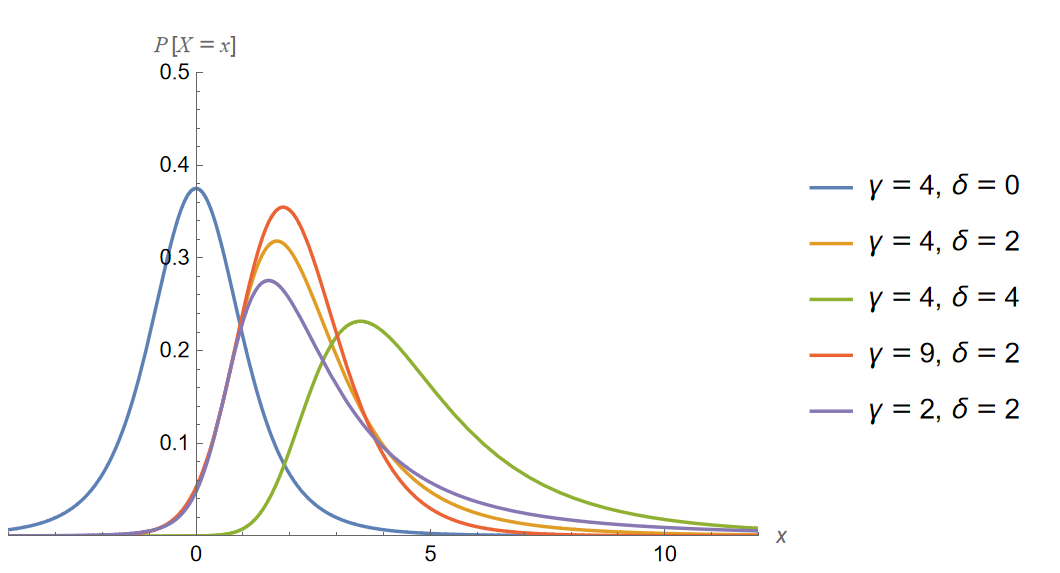
\includegraphics[scale=0.65]{img/pdf_noncentral_t.png}
    \caption{Probability Density Function of Noncentral $T$-Distribution with Various Parameters}
\end{figure}

From the figure we can infer some properties of noncentral $T$-distribution: similar to $T$-distribution, it is uni-modal, but has a skewed behavior towards the direction of non-centrality; and the skewing effect increases as the non-centrality increases. Again similar to $T$-distribution, as the degrees of freedom increases noncentral $T$-distribution behaves more and more like normal distribution with mean the same as the non-centrality. This makes sense as with the sample size increasing, the unbiased estimator for sample variance will have a closer and closer approximation of the actual variance $\sigma^2$, in which case we have exactly the normal distribution.

Using this, we now seek to use this for power analysis. Manipulating the expressions, we have
$$
T_{n-1,\mu\sqrt{n}/\sigma}=\frac{\frac{\Bar{X}-\mu}{\sigma/\sqrt{n}}+\frac{\mu}{\sigma/\sqrt{n}}}{\sqrt{\frac{(n-1)S^2}{\sigma^2}\frac{1}{n-1}}}=\frac{\Bar{X}}{S/\sqrt{n}}
$$
which follows a non-central student T-distributed with $n-1$ degrees of freedom and $\frac{\mu\sqrt{n}}{\sigma}$ non-centrality. That is, if the sample is taken from a batch that does not has mean $\mu$, its distribution will be like this. In this case, we can also interpret $\mu$ as the difference between the actual mean and the mean that we estimate (or the mean that is stated in the null hypothesis).

Since we have obtained the critical region to be
$$
(-\infty, t_{0.995,n-1})
$$
we will calculate $\beta$ as the integral of the noncentral $T$-distribution on the complementary of the critical region, which can be evaluated via
$$
\beta = \int_{-t_{0.005, n-1}}^{\infty} f_{T_{n-1, \frac{\mu\sqrt{n}}{\sigma}}}(x) \d x
$$
As the $\beta$ value is only related to $n$ and the quotient of $\mu$ and $\sigma$, we could express the difference in mean using the multiples of sigma, which gives the Operating Characteristic (OC) Curve as below\footnote{Generated using Mathematica, with source code listed in \ref{mmacode}}:

\begin{figure}[htbp]
    \centering
    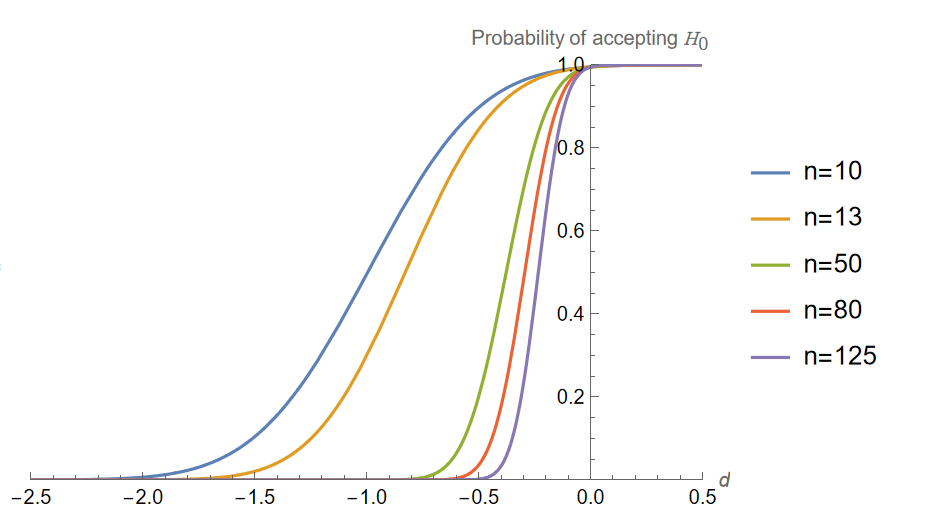
\includegraphics[scale=0.6]{img/oc_noncentral_t.png}
    \caption{OC Curve for One-Tailed Test of Noncentral $T$-Distribution with n Specified in Table 4.3.2}
\end{figure}

\noindent where we have adopted the abscissa to be
$$
d := \dfrac{\mu - \mu_0}{\sigma}
$$
and the ordinate to be the probability of accepting $H_0$ since by definition
$$
P[\text{Accept } H_0] = 1 - P[\text{Reject }H_0]
$$
Without calculating explicitly, we can claim that the test is fairly powerful. Suppose that the non-centrality is of $\sigma$, i.e. the mean of the batch is of shortfall of one standard deviation, for sample size $n\geq 50$ the probability of detecting this is almost 1. Even for the requirement (B.2) that we should spot batches with mean less than or equal to $Q_0 - 0.74\sigma$ ($\delta = Q_0 - 0.74\sigma$), for $n\geq 50$ we can satisfy the requirement as the OC Curve approaches zero. The explicit evaluation of $\beta$ justifies the intuition:

\begin{table}[htbp]
    \centering
    \begin{tabular}{ccc}
        \toprule
        $n$ & $1-\beta\mid\delta = Q_0 - \sigma$ & $1-\beta\mid\delta = Q_0 - 0.74\sigma$ \\
        \midrule
        10 & 0.504 & 0.256 \\
        13 & 0.701 & 0.393 \\
        50 & 1.000 & 0.993 \\
        80 & 1.000 & 1.000 \\
        125 & 1.000 & 1.000 \\
        \bottomrule
    \end{tabular}
    \caption{$\beta$ for Noncentral $T$-Distribution of Different Non-centrality with Varying $n$}
\end{table}

\noindent Note that we table $1-\beta$ instead of $\beta$ to align with the OC Curve. The evaluations give us concrete evidence that the test is pwoerful enough for $n\geq 50$.

\subsection{Why not switching $H_0$ and $H_1$?}

\newpage
\section{Appendix}

\subsection{Appendix A: Source Code for Plotting Functions}
\label{mmacode}

\newpage
    \section{References}
    \begingroup  % Omit the "Reference" Title brought by thebibliography
    \renewcommand{\section}[2]{} 
    \begin{thebibliography}{99}
        \bibitem{Ho2023} Horst Hohberger. Probabilistic Methods in Engineering (lecture slides). University of Michigan - Shanghai Jiao Tong University Joint Institute. Spring 2023. (An earlier version can be found at \href{http://ece401.ji.sjtu.edu.cn/ewExternalFiles/ve401\_all\_lecture\_slides.pdf}{http://ece401.ji.sjtu.edu.cn/ewExternalFiles/ve401\_all\_lecture\_slides.pdf})
        \bibitem{JJF2005} AQSIQ/MTC1. Rules of metrological testing for net quantities of products in prepackages with fixed content. Technical Report JJF 1070-2005, Chinese Metrology Press, 2005. Available from \href{http://www.gdifi.org.cn/spbz/437.jhtml}{http://www.gdifi.org.cn/spbz/437.jhtml} [Online; accessed 17-April-2023].
		\bibitem{OIML2016} Quantity of product in prepackages. Technical Report OIML R 87, International Organization of Legal Metrology (OIML), 2016. Available from \href{https://www.oiml.org/en/files/pdf\_r/r087-e16.pdf}{https://www.oiml.org/en/files/pdf\_r/r087-e16.pdf} [Online; accessed 25-March-2023].
        \bibitem{Wi2023} Wikipedia. Noncentral t-distribution — wikipedia, the free encyclopedia, 2014. \href{https://en.wikipedia.org/wiki/Noncentral\_t-distribution}{https://en.wikipedia.org/wiki/Noncentral\_t-distribution} [Online; accessed 10-April-2014].
    \end{thebibliography}
    \endgroup

\end{document}

